\section{TP2: LCD Time}
\subsection{Objectif}
Dans cette manipulation nous allons apprendre a utiliser un ecran LCD\@. Nous commencerons par decouvrir comment ecrire des phrases simples, puis nous afficherons un texte defillant et enfin nous utiliserons des variables pour afficher l'heure.
\subsection{Matériel}
\begin{itemize}
	\item Un ordinateur
	\item Un arduino Uno R3
	\item Un ecran LCD
	\item Une resistance de 10K$\Omega$
	\item Un potentiometre
\end{itemize}

\subsection{Nom-Prenom}
Le montage est identique pour toutes les manipulations de ce labo. Nous avons utilise la librairie LiquidCrystal, disponnible sur le site officiel d'Arduino. Ici nous allons écrire nos noms sur chacune des lignes de l'écran LCD avec, à gauche, le numéro de notre groupe. Nous utilsons la librairie LiquidCrystal qui nous permet de facilement afficher du texte sur notre écran LCD\@.
\lstinputlisting[language=C]{Code/TP2/TP2.1/TP2.1.ino}
\begin{figure}[H]
	\centering
	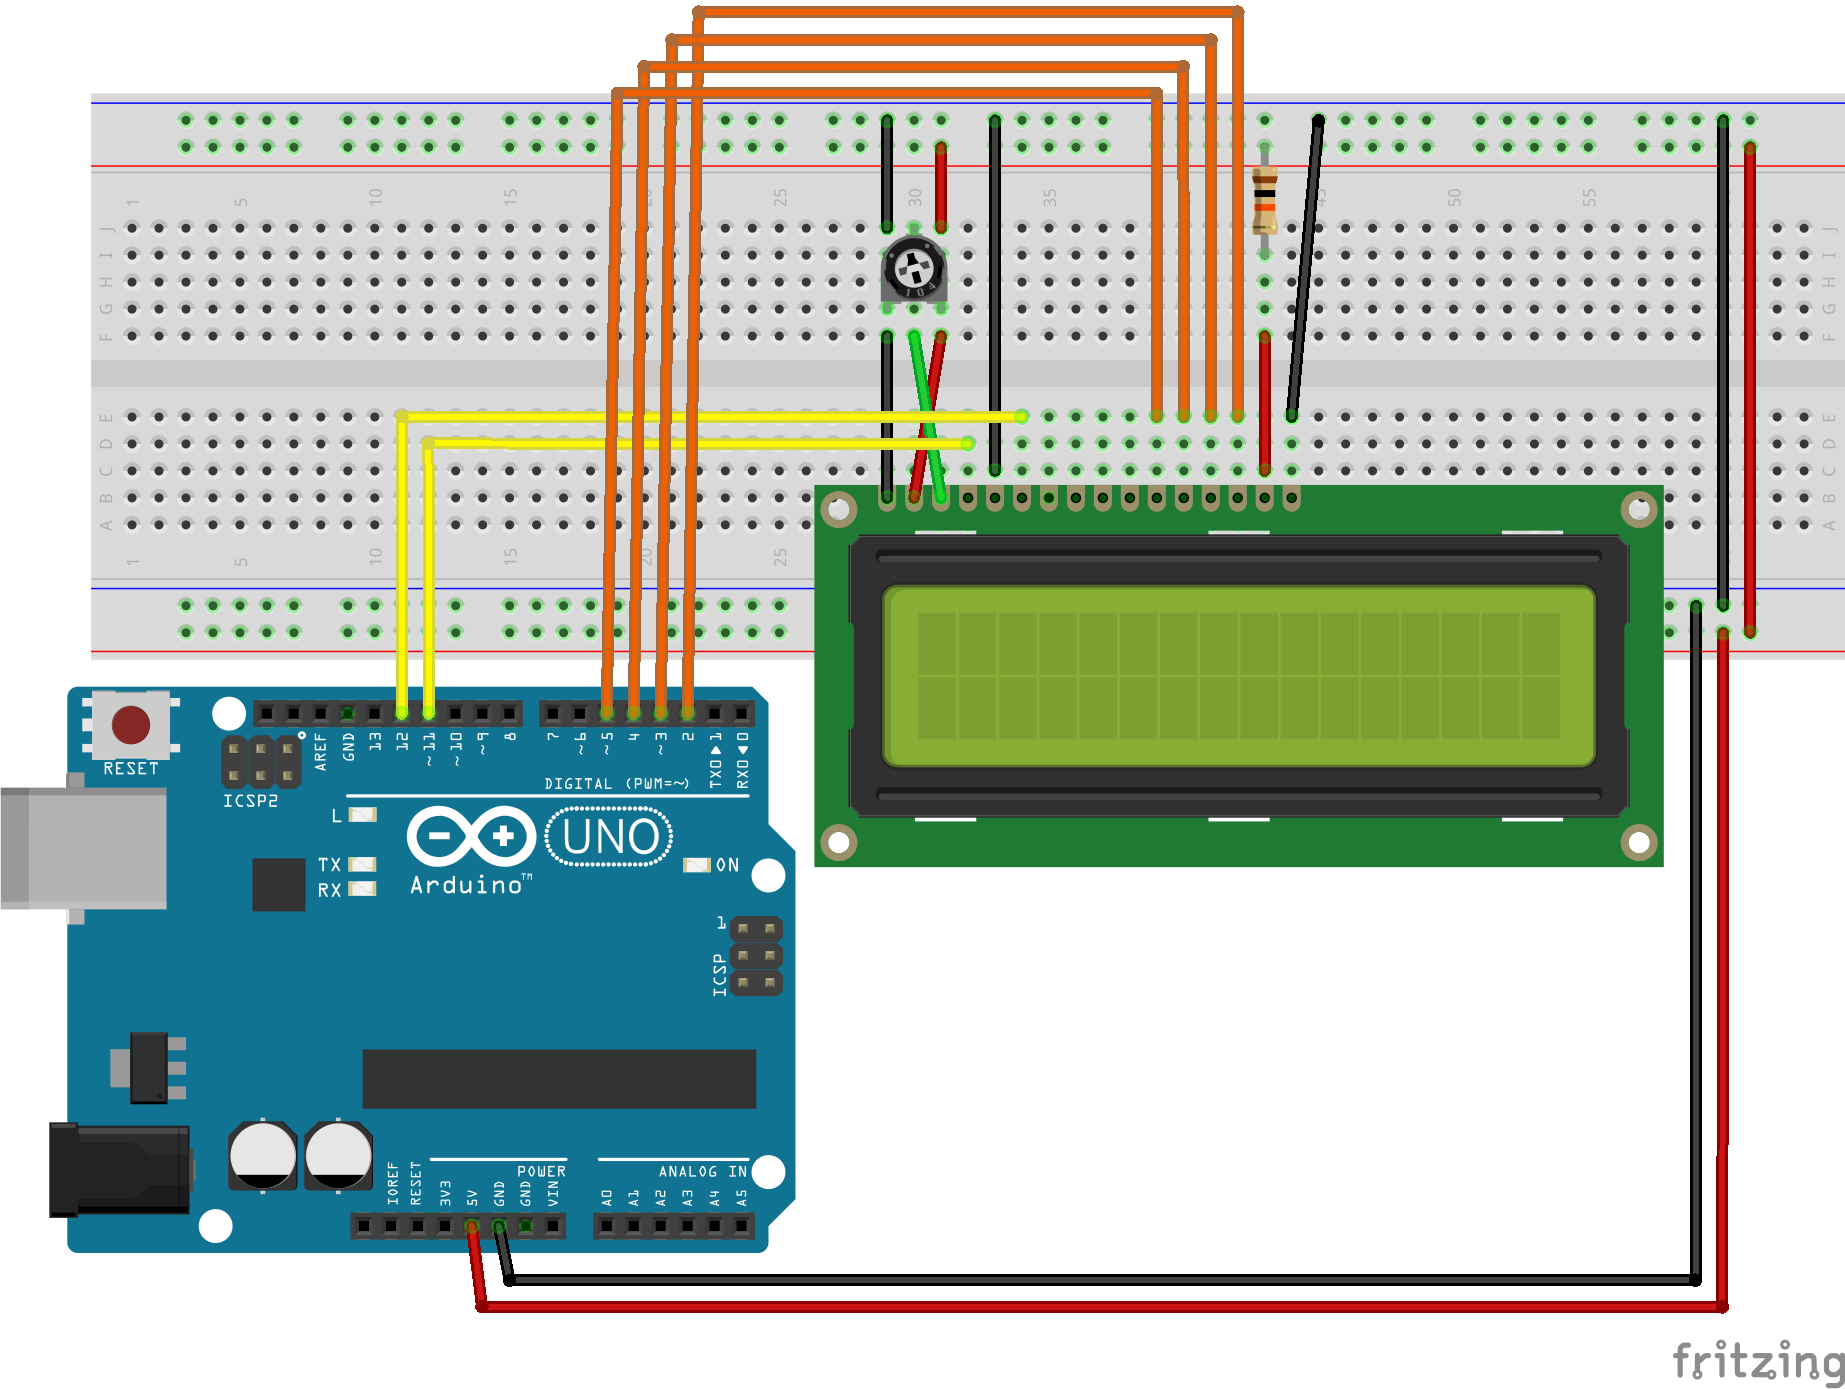
\includegraphics[height=6cm]{img/TP2-1.png}
	\caption{\label{TP2.1}Nom-Prenom}
\end{figure}
%TODO Ecran LCD

\subsection{Texte deroulant}
Dans cette manipulation nous allons afficher un texte déroulant vers la gauche.
\lstinputlisting[language=C]{Code/TP2/TP2.2/TP2.2.ino}

\subsection{Horloge}
Dans cette manipulation nous allons afficher une horloge au milieu de la deuxième ligne de l'écran. Une fois téléversé, l'Arduino commencera a afficher l'heure à 22h59m50 car il n'est pas possible d'afficher l'heure réelle sans utiliser des boutons pour régler l'heure ou un module \textit{Real Time Clock}.
\lstinputlisting[language=C]{Code/TP2/TP2.3/TP2.3.ino}

\subsection{Decompte}
De la même façon que nous avons affiché l'heure nous affichons ici un décompte qui part de 9999 jusu'à 0.
\lstinputlisting[language=C]{Code/TP2/TP2.4/TP2.4.ino}
